\section{Elasto-Plastic Dynamic Response Analysis}

\subsection{Problem Definition}

The system considered in Question 1 is now assumed to exhibit a perfectly elasto-plastic force-displacement relationship with yield force:

\begin{equation}
F_y = 24 \ \text{kN} = 24000 \ \text{N}
\end{equation}

The equation of motion becomes:

\begin{equation}
m\ddot{u}(t) + c\dot{u}(t) + F_r(t) = F(t)
\end{equation}

where $F_r(t)$ is the nonlinear restoring force.



\subsection{Elasto-Plastic Constitutive Model}

The restoring force is modeled as perfectly elasto-plastic in terms of elastic and plastic displacement components:

\begin{equation}
u = u_e + u_p, \qquad F_r = k u_e = k(u-u_p)
\end{equation}

At each step, a trial restoring force is formed from the previous plastic displacement:

\begin{equation}
F_{\text{trial}} = k\left(u_{n+1}^{\text{trial}} - u_{p,n}\right)
\end{equation}

The return-mapping rule is:

\begin{equation}
F_{r,n+1} =
\begin{cases}
k\left(u_{n+1} - u_{p,n}\right), & |F_{\text{trial}}| \leq F_y \\
\pm F_y, & |F_{\text{trial}}| > F_y
\end{cases}
\end{equation}

with plastic displacement update in the yielded state:

\begin{equation}
u_{p,n+1} = u_{n+1} - \frac{F_{r,n+1}}{k}
\end{equation}

where:
\begin{itemize}
\item $u_p$ is the plastic displacement,
\item $k$ is the elastic stiffness,
\item $F_y$ is the yield force.
\end{itemize}

The yield displacement is:

\begin{equation}
u_y = \frac{F_y}{k}
\end{equation}



\subsection{Numerical Solution Procedure}

The nonlinear dynamic response is computed using a step-by-step incremental
direct integration algorithm, as illustrated in Figure X. The method advances
the solution in time without iteration by updating the system state at each
time step based on the tangent stiffness and equilibrium conditions.

The governing equation is:
\begin{equation}
m \ddot{u} + c \dot{u} + F_s(u) = F(t)
\end{equation}

First, the initial acceleration is obtained from equilibrium:
\begin{equation}
\ddot{u}_0 = \frac{1}{m}\left(F_0 - c\dot{u}_0 - F_s(u_0)\right)
\end{equation}

At each time step $i$, the following procedure is applied:

\begin{enumerate}
\item Compute the effective stiffness:
\begin{equation}
k_i^* = k_i(u_i) + \frac{2c}{\Delta t} + \frac{4m}{\Delta t^2}
\end{equation}

\item Compute the effective force increment:
\begin{equation}
\Delta F_i^* = \Delta F_i + \left(\frac{4m}{\Delta t} + 2c\right)\dot{u}_i + 2m \ddot{u}_i
\end{equation}

\item Solve for the displacement increment:
\begin{equation}
\Delta u_i = \frac{\Delta F_i^*}{k_i^*}
\end{equation}

\item Compute velocity and acceleration increments:
\begin{align}
\Delta \dot{u}_i &= \frac{2}{\Delta t}\Delta u_i - 2\dot{u}_i \\
\Delta \ddot{u}_i &= \frac{4}{\Delta t^2}\Delta u_i - \frac{4}{\Delta t}\dot{u}_i - 2\ddot{u}_i
\end{align}

\item Update displacement and velocity:
\begin{align}
u_{i+1} &= u_i + \Delta u_i \\
\dot{u}_{i+1} &= \dot{u}_i + \Delta \dot{u}_i
\end{align}

\item Evaluate the restoring force $F_{s,i+1}$ using the elasto-plastic
constitutive model and update the plastic displacement.

\item Compute the acceleration from dynamic equilibrium:
\begin{equation}
\ddot{u}_{i+1} = \frac{F_{i+1} - c\dot{u}_{i+1} - F_{s,i+1}}{m}
\end{equation}

\item Advance to the next time step and repeat.
\end{enumerate}

This formulation allows the nonlinear response to be obtained efficiently
without iterative correction within each time step, while maintaining
consistency with the governing dynamic equilibrium.


\subsection{Results}

The displacement, velocity, and acceleration time histories for both linear and elasto-plastic cases are shown below.

\begin{figure}[h]
\centering
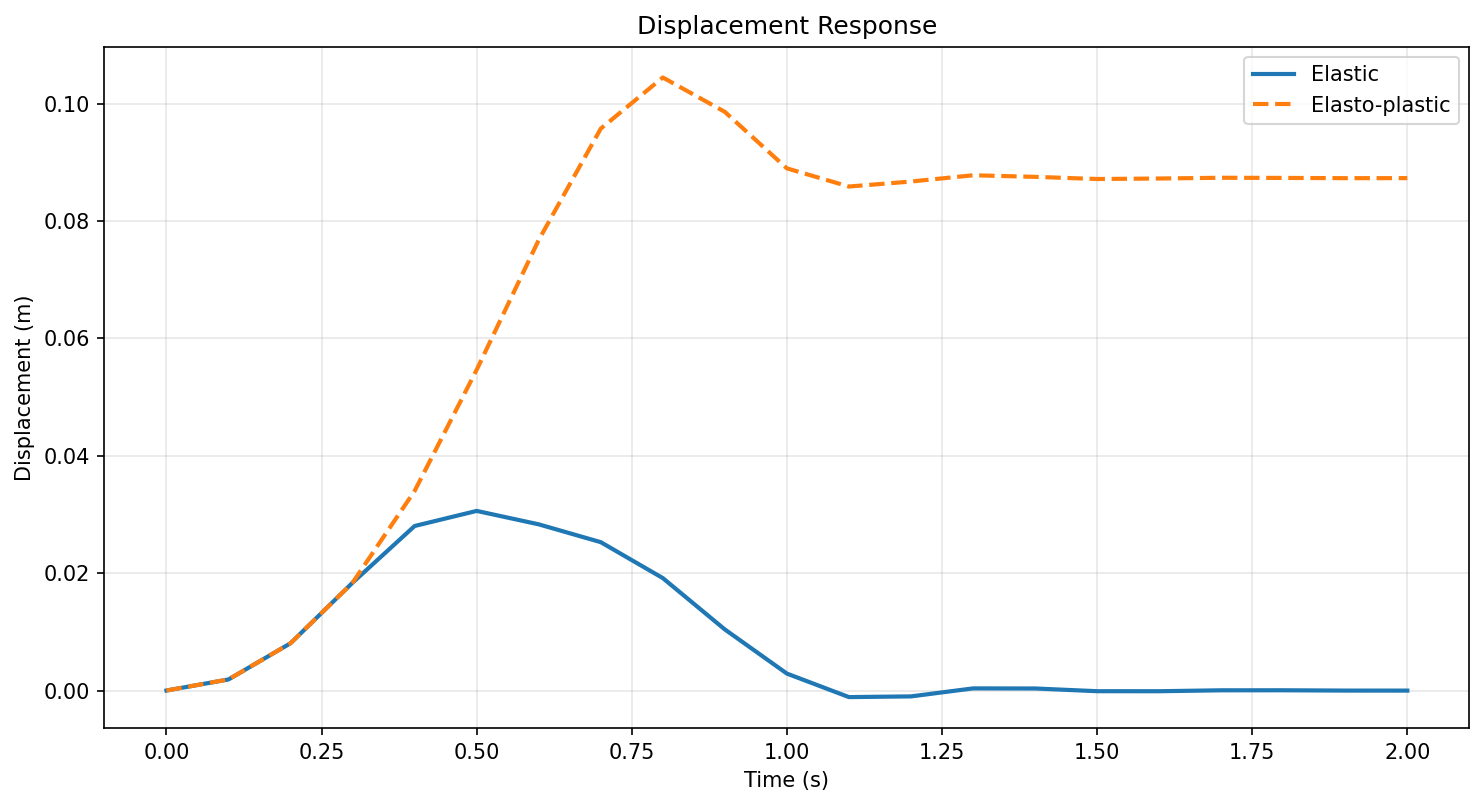
\includegraphics[width=0.8\textwidth]{figures/plastic_displacement_inelastic.png}
\caption{Displacement response comparison}
\end{figure}

\begin{figure}[h]
\centering
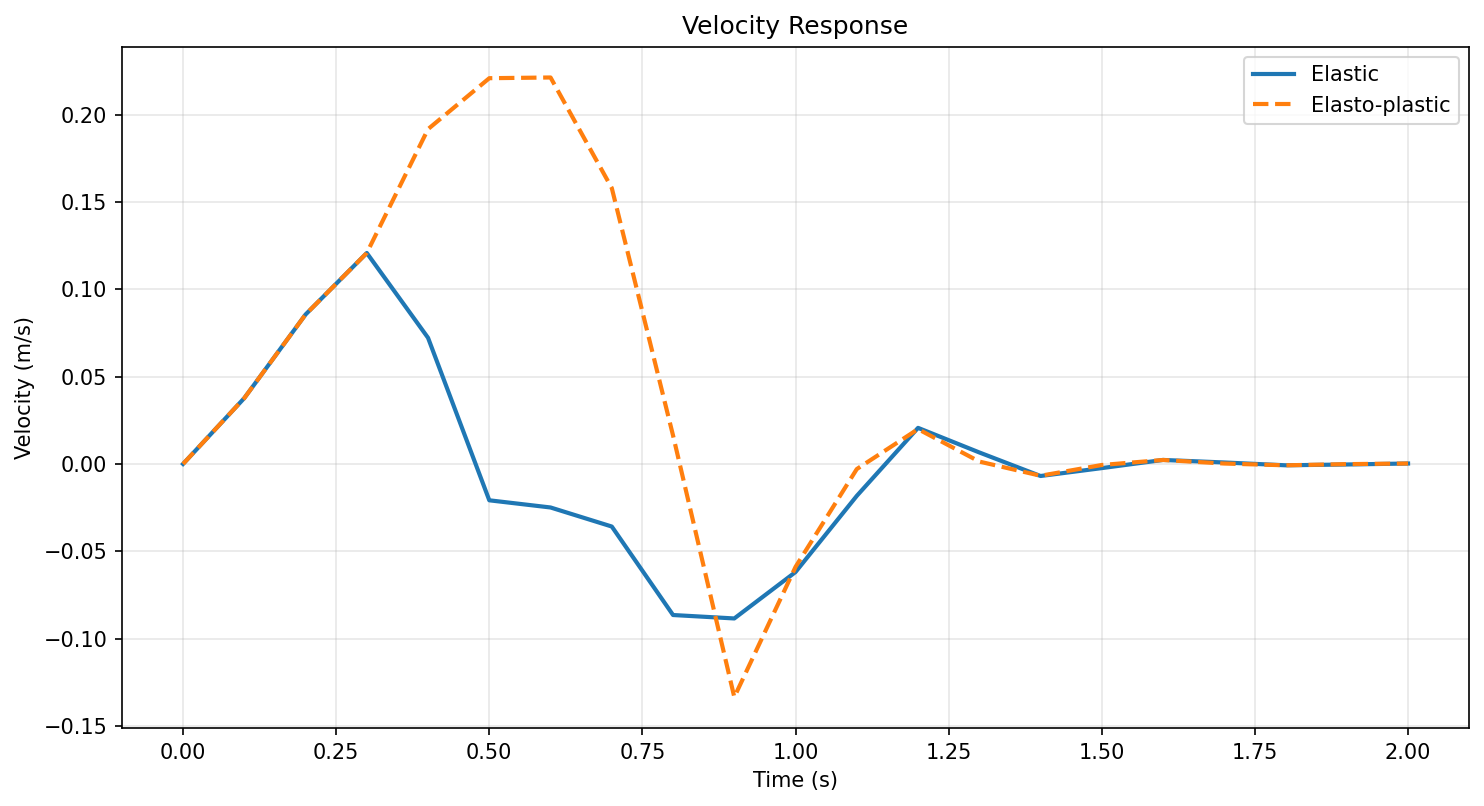
\includegraphics[width=0.8\textwidth]{figures/plastic_velocity_inelastic.png}
\caption{Velocity response comparison}
\end{figure}

\begin{figure}[h]
\centering
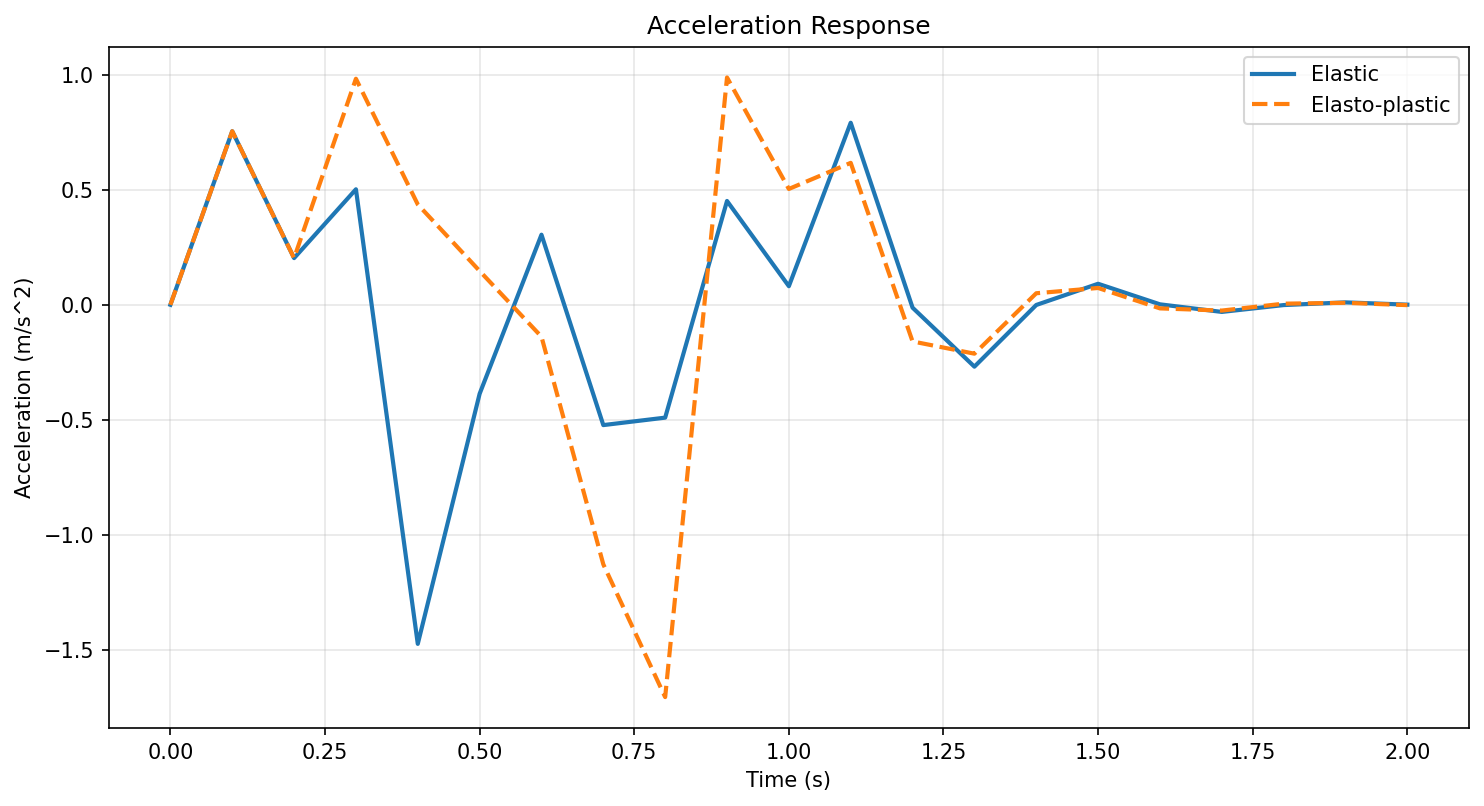
\includegraphics[width=0.8\textwidth]{figures/plastic_acceleration_inelastic.png}
\caption{Acceleration response comparison}
\end{figure}



\subsection{Force--Displacement Relationship}

The force-displacement relationship for both cases is shown in Figure below. The elastic reference line is drawn only up to the yield force level ($\pm F_y$) for a consistent comparison with the elasto-plastic response.

\begin{figure}[h]
\centering
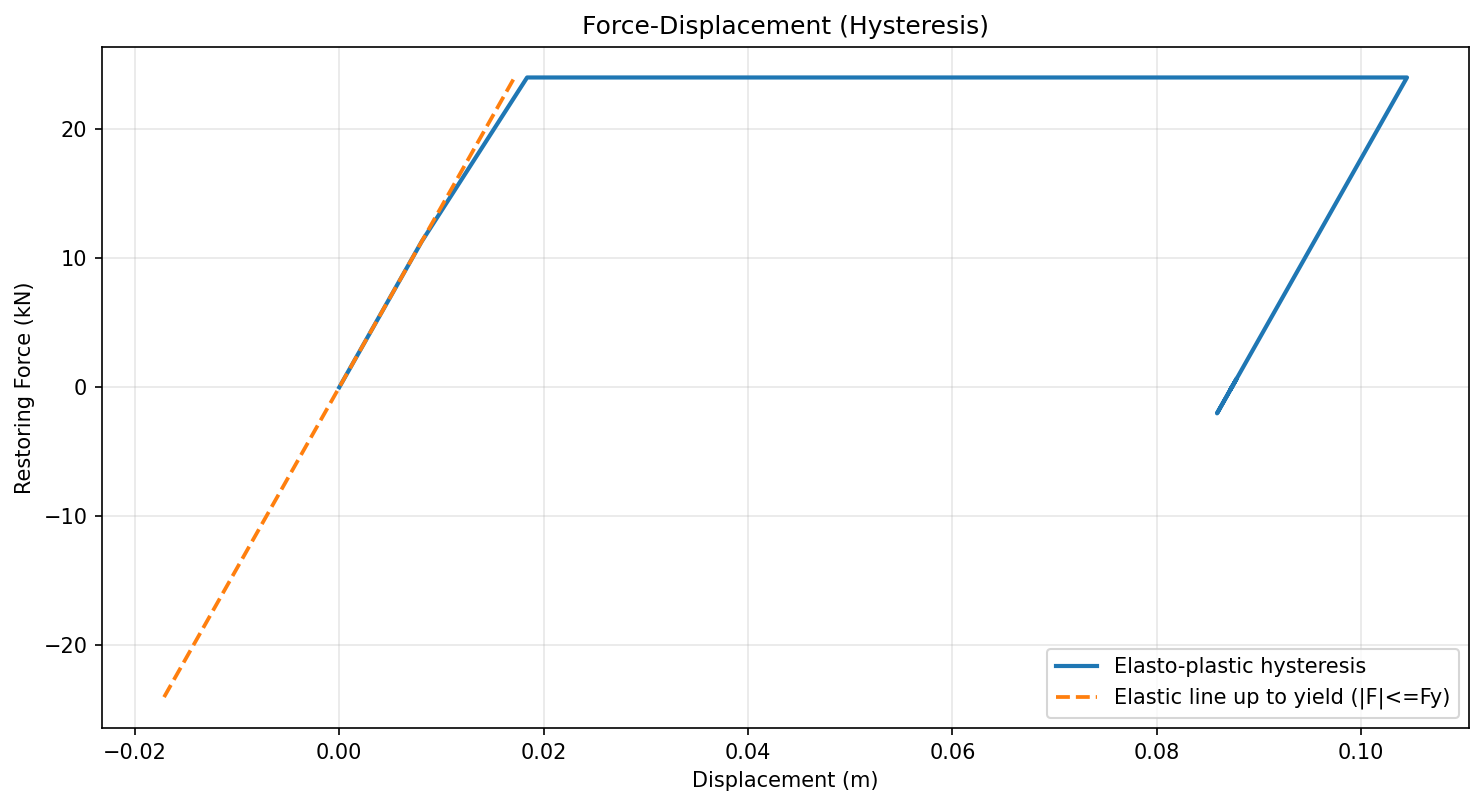
\includegraphics[width=0.8\textwidth]{figures/force_displacement_hysteresis.png}
\caption{Force-displacement relationship (elastic vs elasto-plastic)}
\end{figure}



\subsection{Discussion}

The elasto-plastic system exhibits significantly different behavior compared to the linear-elastic system.

\begin{itemize}
\item \textbf{Increased displacement:} After yielding, the effective stiffness reduces, leading to larger displacements.
\item \textbf{Force limitation:} The restoring force is capped at $\pm F_y$, preventing further force increase.
\item \textbf{Energy dissipation:} Plastic deformation dissipates energy, reducing oscillation amplitudes.
\item \textbf{Residual displacement:} Unlike the elastic system, the elasto-plastic system does not return to zero displacement after loading ceases.
\end{itemize}

The hysteresis loop clearly illustrates the nonlinear behavior and energy dissipation mechanism.



\subsection{Summary of Results}

\begin{itemize}
\item Maximum displacement in the elasto-plastic system is greater than that of the elastic system.
\item The restoring force remains bounded within $\pm F_y$.
\item Residual displacement is observed at the end of the simulation.
\item Equilibrium residuals after convergence are near numerical precision.
\end{itemize}

\subsection{Latest Script Output (Incremental Direct Integration)}

The nonlinear solver was executed with the CE586 incremental direct integration algorithm and the following outputs were obtained:

\begin{itemize}
\item Yield displacement: $u_y = F_y/k = 1.714286 \times 10^{-2}\ \mathrm{m}$
\item Restoring force cap check: $\max |F_s| = 24000.000000\ \mathrm{N} \le 24000.000001\ \mathrm{N}$ (Pass)
\item Peak elastic displacement: $\max |u_{\mathrm{elastic}}| = 3.060777 \times 10^{-2}\ \mathrm{m}$
\item Peak inelastic displacement: $\max |u_{\mathrm{inelastic}}| = 1.044710 \times 10^{-1}\ \mathrm{m}$
\item Distinct response check: $\max |u_{\mathrm{inelastic}}-u_{\mathrm{elastic}}| = 8.820017 \times 10^{-2}\ \mathrm{m}$ (Pass)
\item Residual displacement at $t=2.0\,\mathrm{s}$: $8.731893 \times 10^{-2}\ \mathrm{m}$
\item Max restoring force: $24000.00\ \mathrm{N}$
\item Max equilibrium residual:
$$\max |F - m a - c v - F_s| = 1.819 \times 10^{-12}\ \mathrm{N}$$
\end{itemize}